% !TeX spellcheck = de_DE

\chapter{Entwurf}
\label{chap:entwurf}

Während in der Spezifikation noch auf den zu erstellenden Prototypen eingegangen wurde, protokolliert der Entwurf die Designentscheidungen und Struktur der zu erstellenden Software.

\section{Einleitung}

\subsection{Zweck des Entwurfs}
Der Entwurf bietet den Entwicklern ein Grundgerüst, das als Orientierung der Software dienen soll.
Es werden alle grundlegenden Entscheidungen \bzgl der Struktur der Software festgehalten.
Hierbei werden das Gesamtsystem, sowie einzelne Komponenten detailliert mit Hilfe von UML-Diagrammen beschrieben.
Durch das Dokument soll auch den zukünftigen Software-Entwicklern die Wartung der Software erleichtert werden.

\subsection{Lesekreis des Entwurfs}
Folgende Personen gehören zum Leserkreis dieses Dokuments:
\begin{itemize}
	\item Der Kunde
	\item Das gesamte Entwicklerteam
	\item Die universitären Betreuer
\end{itemize}

\subsection{Überblick über das Entwurfsdokument}
Zunächst werde in Kapitel 2 die grundsätzliche Entwurfsentscheidungen beschrieben.

In Kapitel 3 werden die einzelnen Komponente detailliert beschrieben.

\subsection{Schreibweisen und Abkürzungen}
Paketnamen werden im Dokument \textbf{fett} hervorgehoben. Klassennamen werden \textit{kursiv} dargestellt.

Bei eventuell unklaren Fachbegriffen und Abkürzungen, ist im Begriffslexikon der Spezifikation \bzw der Spezifikation selbst eine Erklärung zu selbigen zu finden.

\subsection{Aufbau dieses Dokuments}
Zunächst sollen allgemeine Entwurfsentscheidungen, wie verwendete Entwurfs- und Architekturmuster erläutert werden.
Dies soll ein Überblick über die grundsätzliche Struktur und Vorgehensweise im Entwurf verschaffen.
Im darauffolgenden Kapitel werden die Komponenten mit ihren Paketen und Klassen detailliert beschrieben.

\subsection{Einschränkungen in der Technik}
Die Implementierung muss in C\# 5 erfolgen.
Zusätzlich müssen die SDKs der Kameras bestmöglich benutzt werden.

\section{Grundsätzliche Entwurfsentscheidungen}

\subsection{Entworfene Software und Anforderung an den Entwurf}
Die Software soll die Bilder einer Wärmebildkamera oder Tiefenbildkamera anzeigen und in beiden Bildern soll zusätzlich die Distanz zum Objekt im Mittelpunkt des Bildes angezeigt werden.
Außerdem soll die Software bei Kamerabilder überlagern, sodass man Kanten des überstrahlten Objektes nachzeichnen kann und die Entfernungen bestimmen kann.

Die zu entwickelnde Systemsoftware ist ein Einbenutzersystem, welches dementsprechend mehrmals parallel ausgeführt werden kann, aber jeweils immer nur von einem Nutzer bedient werden kann.

Alle in diesem Dokument getroffenen Entwurfsentscheidungen orientieren sich an den oben genannten Funktionen der Software, die in der Spezifikation genauer beschrieben sind.

Der Entwurf berücksichtigt im Besonderen die nicht-funktionalen Anforderungen, wie Test-, Wart-, Portier- und Erweiterbarkeit des Systems.

\subsection{Entwurfsmuster und allgemeine Prinzipien}
Es werden folgende Entwurfsmuster verwendet:
\begin{description}
	\item [Adapter] --- Übersetzung einer Schnittstelle zu einer anderen.
\end{description}

Allgemein soll eine möglichst lose Kopplung zwischen den Modulen und ein hoher Zusammenhalt innerhalb von Klassen und Paketen herrschen.

\subsection{Hardwareansicht}
Im folgenden soll eine Übersicht über die beteiligten Geräte und deren Verbindungen untereinander gegeben werden.

Die Kameras und die Brille sind über einen USB-Port an dem Laptop angeschlossen, während der Laptop via WLAN mit dem Smartphone kommuniziert.
\begin{figure}[H]
		\centering
		\ifthenelse{\boolean{jpg}}{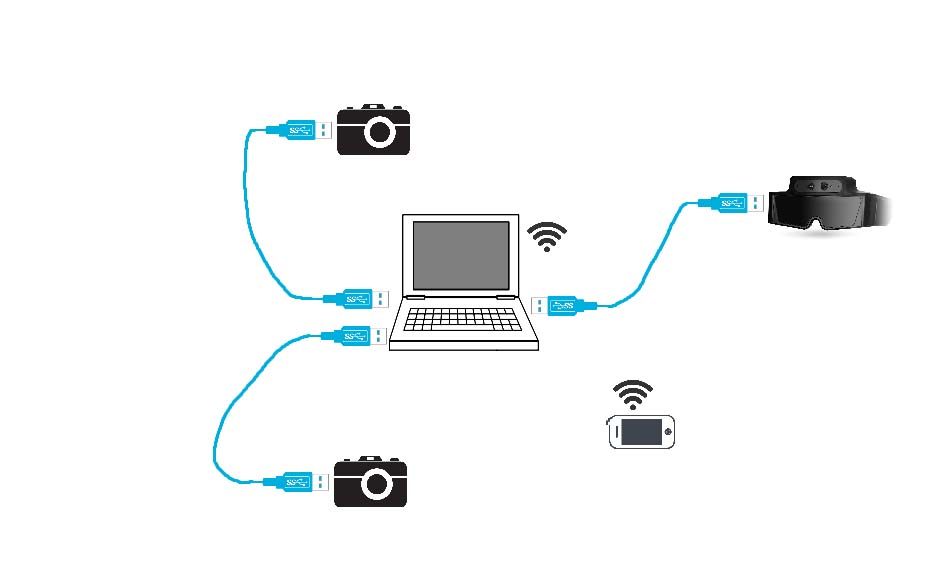
\includegraphics[width=\textwidth]{Entwurf/Hardware_Entwurf.jpg}}{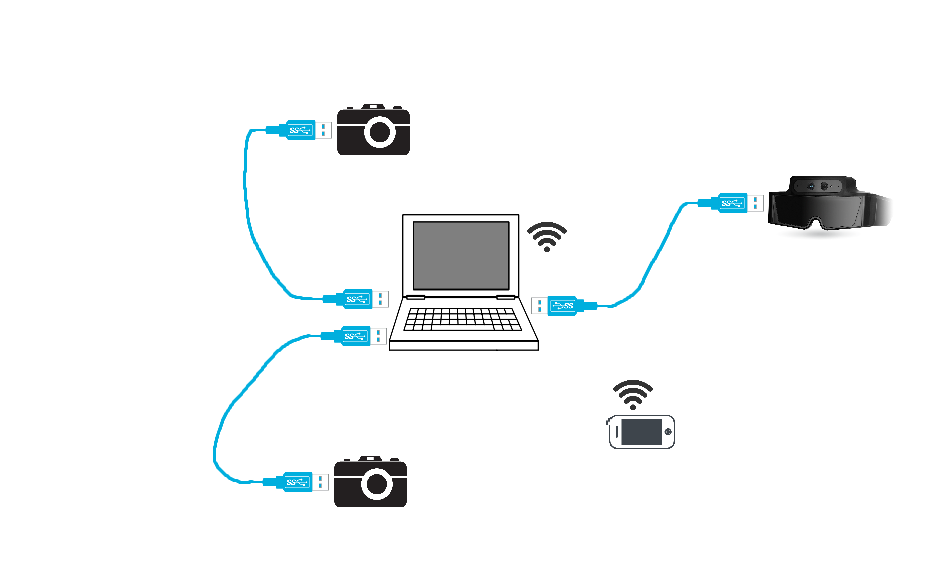
\includegraphics[width=\textwidth]{Entwurf/Hardware_Entwurf.png}}
		\caption{Hardwareaufbau}
		\label{fig:entwurf_hardware}
\end{figure}

\subsection{Komponentendiagramm}
Das Komponentendiagramm bietet eine grobe Übersicht, über die geplanten Interaktionen der Komponenten untereinander.
Eine genauere Beschreibung der einzelnen Komponenten erfolgt im Paketdiagramm.
\begin{figure}[H]
	\centering
	\ifthenelse{\boolean{jpg}}{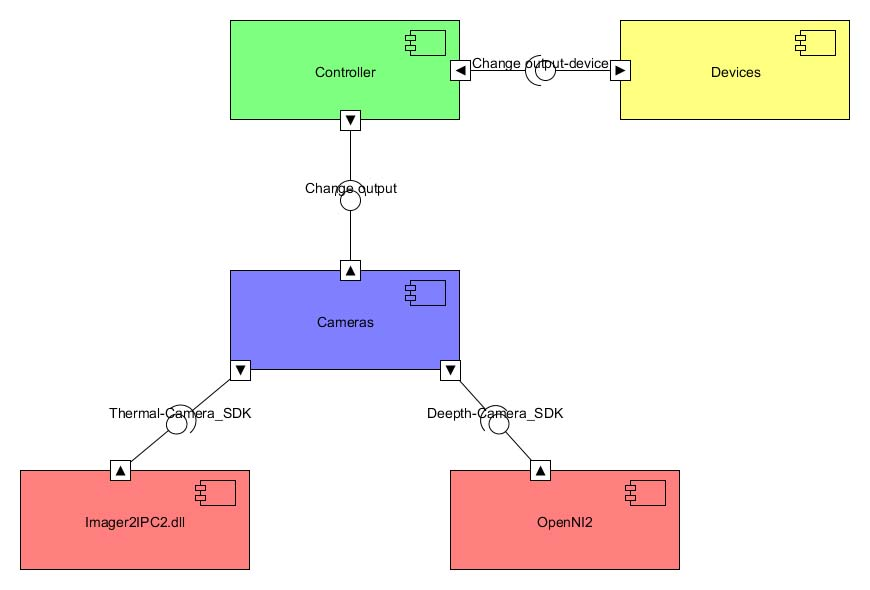
\includegraphics[width=\textwidth]{Entwurf/Komponenten.jpg}}{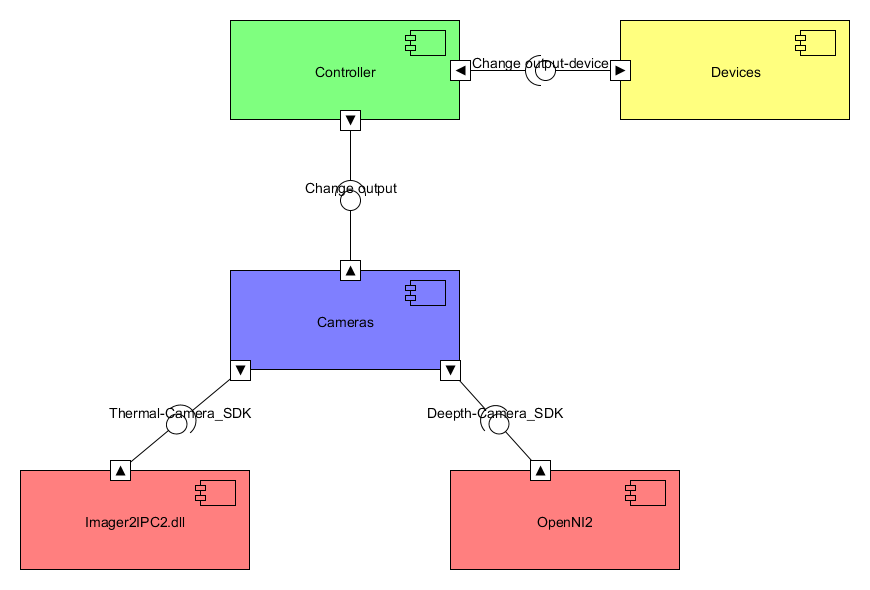
\includegraphics[width=\textwidth]{Entwurf/Komponenten.png}}
	\caption{Komponentendiagramm}
	\label{fig:entwurf_komponenten}
\end{figure}

\section{Beschreibung der einzelnen Komponenten}
Die Komponente Controller ist für den Programmfluss und das Benutzermenü mitsamt Interaktion zuständig.

Die Cameras-Komponente ist der Adapter für die externen Bibliotheken.
Alle bilderstellende und informationsgenerierende Bestandteile sind in dieser Komponente enthalten.

Die Devices-Komponente ist für den Umgang mit allen Ausgabegeräten verantwortlich.
Sämtliche Hardware-Interaktion mit nicht bilderstellenden Geräten wird hier geregelt.

Sowohl die Imager2IPC2 als auch die OpenNI2 Komponente sind externe Bibliotheken, die zur Bilderstellung benötigt werden.

\subsection{Die Komponenten Cameras, Controller und Devices}
\subsubsection{Paketdiagramm}
Das Paketdiagramm verschafft einen Überblick über die in den Komponenten vorkommenden Pakete.
Die einzelnen Pakete werden durch ihre Klassen und deren Methoden spezifiziert.

Während das \textbf{Controller}-Paket Zugriff auf ausgewählte Teile von \textbf{Devices} und \textbf{Camera.net} hat, können diese nicht auf Teile von Controller zugreifen.
Zwischen \textbf{Devices} und \textbf{Camera.net} stehen in keiner Beziehung zueinander.

\textbf{Camera.net} importiert zusätzlich allerdings Funktionen aus den gegebenen Bibliotheken \textbf{Camera SDK}.
Logischerweise ist dies eine einseitige Beziehung.

Damit ist eine hierarchische Ordnung gegebenen.
\begin{figure}[H]
	\centering
	\ifthenelse{\boolean{jpg}}{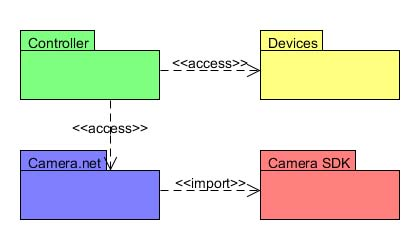
\includegraphics[width=0.6\textwidth]{Entwurf/Paket.jpg}}{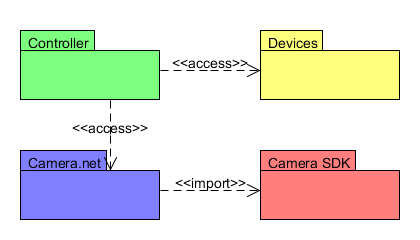
\includegraphics[width=0.6\textwidth]{Entwurf/Paket.png}}
	\caption{Paketdiagramm}
	\label{fig:entwurf_paket}
\end{figure}

\subsubsection{Klassendiagramm}
Das Klassendiagramm dient zur Veranschaulichung der einzelnen Beziehungen zwischen den Paketen und ihren Klassen.
\begin{figure}[H]
	\centering
	\ifthenelse{\boolean{jpg}}{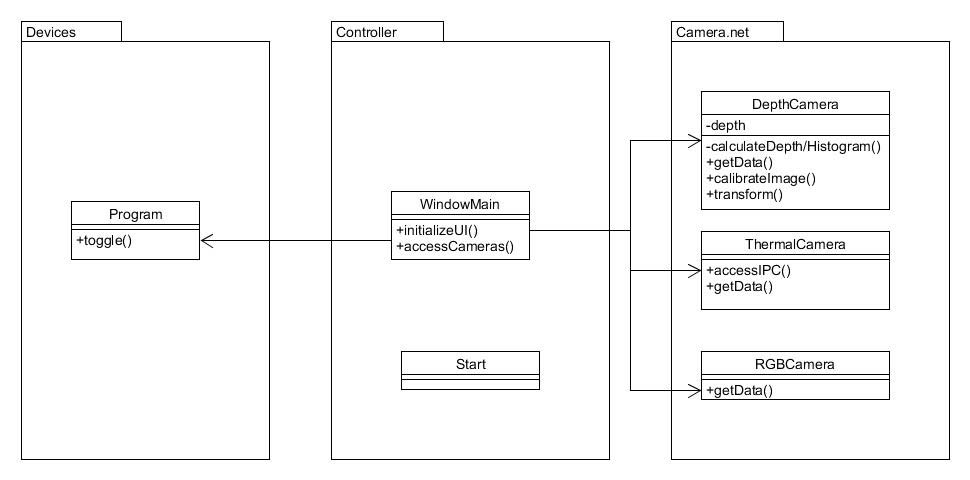
\includegraphics[width=\textwidth]{Entwurf/Klassen.jpg}}{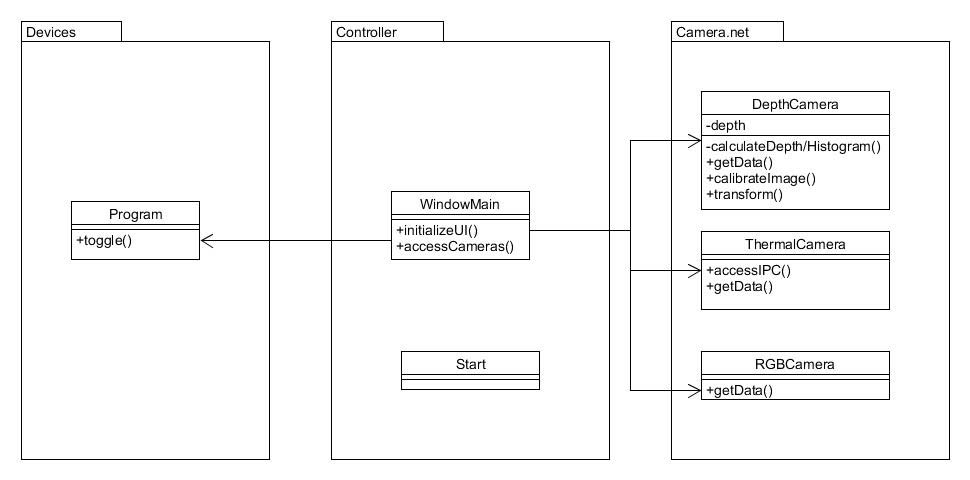
\includegraphics[width=\textwidth]{Entwurf/Klassen.jpg}}
	\caption{Klassendiagramm}
	\label{fig:entwurf_class}
\end{figure}

\subsubsection{Beschreibung}
Die Komponente \textbf{Cameras} besteht aus den Klassen \textit{DepthCamera}, \textit{ThermalCamera}, \textit{RGBCamera}.
Die Klasse \textit{DepthCamera} ist für die Generierung der Tiefenbilder zuständig.
Die Klasse \textit{ThermalCamera} für die Generierung der Wärmebilder verantwortlich.
Zusätzlich wird die Temperatur des Bildmittelpunktes gemessen und der \textit{Viewer}-Klasse zu Verfügung gestellt.
In diesen beiden Klassen können auf die jeweiligen Informationen zugegriffen werden.

Die Klasse \textit{RGBCamera} ist für die Generierung des RGB-Bilds zuständig.

Das Paket \textbf{Controller} besteht aus den Klassen \textit{Form} und \textit{Start}.

Die Klasse \textit{WindowMain} ist zuständig für die Erstellung, Anzeige und Bedienung der Benutzeroberfläche.
Alle auswählbaren Optionen werden von hier aus an die zuständigen Objekte weitergereicht.

Die Klasse \textit{Start} ist zuständig für die Ausführung des Programms und dafür verantwortlich, dass zum Programmstart die gewünschten Windows-Einstellungen gesetzt, sowie zum Programmende die alten wiederhergestellt werden.

Die Klasse \textit{Monitor} ist eine abstrakte Klasse, die die Grundfunktionen jedes Ausgabegerätes enthält.
Dazu gehört das Aktivieren und Deaktivieren eines Ausgabegeräts.

\subsection{Externe Komponenten}
Für die Generierung der Tiefenbilder wird das SDK OpenNI verwendet.
Für die Generierung der Wärmebilder wird die Bibliothek Imager2IPC.dll verwendet.

\section{Versionhistorie}
\begin{description}
	\item [Version 1.0 (27.7.2015)] Erstellung des Dokuments
	\item [Version 1.1 (9.8.2015)] Spezifizierung der Klassen
	\item [Version 1.2 (20.3.2016)] Korrektur des Klassendiagramms
\end{description}